\documentclass[12pt,oneside]{uhthesis}
\usepackage{subfigure}
\usepackage[ruled,lined,linesnumbered,titlenumbered,algochapter,spanish,onelanguage]{algorithm2e}
\usepackage{amsmath}
\usepackage{cite}
\usepackage{amssymb}
\usepackage{amsbsy}
\usepackage{caption,booktabs}
\captionsetup{ justification = centering }
%\usepackage{mathpazo}
\usepackage{float}
\setlength{\marginparwidth}{2cm}
\usepackage{todonotes}
\usepackage{listings}
\usepackage{xcolor}
\usepackage{multicol}
\usepackage{graphicx}
\floatstyle{plaintop}
\restylefloat{table}
\addbibresource{Bibliography.bib}
% \setlength{\parskip}{\baselineskip}%
\renewcommand{\tablename}{Tabla}
\renewcommand{\listalgorithmcfname}{Índice de Algoritmos}
%\dontprintsemicolon
\SetAlgoNoEnd

\definecolor{codegreen}{rgb}{0,0.6,0}
\definecolor{codegray}{rgb}{0.5,0.5,0.5}
\definecolor{codepurple}{rgb}{0.58,0,0.82}
\definecolor{backcolour}{rgb}{0.95,0.95,0.92}

\lstdefinestyle{mystyle}{
    backgroundcolor=\color{backcolour},   
    commentstyle=\color{codegreen},
    keywordstyle=\color{purple},
    numberstyle=\tiny\color{codegray},
    stringstyle=\color{codepurple},
    basicstyle=\ttfamily\footnotesize,
    breakatwhitespace=false,         
    breaklines=true,                 
    captionpos=b,                    
    keepspaces=true,                 
    numbers=left,                    
    numbersep=5pt,                  
    showspaces=false,                
    showstringspaces=false,
    showtabs=false,                  
    tabsize=4
}

\lstset{style=mystyle}

\title{Título de la tesis}
\author{\\\vspace{0.25cm}Nombre del autor}

\hypersetup{
	colorlinks=true,
	linkcolor=blue,
	filecolor=magenta,      
	urlcolor=cyan,
	pdftitle={Overleaf Example},
	pdfpagemode=FullScreen,
}

\advisor{\\\vspace{0.25cm}Nombre del primer tutor\\\vspace{0.2cm}Nombre del segundo tutor}
\degree{Licenciado en (Matemática o Ciencia de la Computación)}
\faculty{Facultad de Matemática y Computación}
\date{Fecha\\\vspace{0.25cm}\href{https://github.com/username/repo}{github.com/username/repo}}
\logo{Graphics/uhlogo}
\makenomenclature

\renewcommand{\vec}[1]{\boldsymbol{#1}}
\newcommand{\diff}[1]{\ensuremath{\mathrm{d}#1}}
\newcommand{\me}[1]{\mathrm{e}^{#1}}
\newcommand{\pf}{\mathfrak{p}}
\newcommand{\qf}{\mathfrak{q}}
%\newcommand{\kf}{\mathfrak{k}}
\newcommand{\kt}{\mathtt{k}}
\newcommand{\mf}{\mathfrak{m}}
\newcommand{\hf}{\mathfrak{h}}
\newcommand{\fac}{\mathrm{fac}}
\newcommand{\maxx}[1]{\max\left\{ #1 \right\} }
\newcommand{\minn}[1]{\min\left\{ #1 \right\} }
\newcommand{\lldpcf}{1.25}
\newcommand{\nnorm}[1]{\left\lvert #1 \right\rvert }
\renewcommand{\lstlistingname}{Ejemplo de código}
\renewcommand{\lstlistlistingname}{Ejemplos de código}

\begin{document}

\frontmatter
\maketitle

\include{FrontMatter/Dedication}
\include{FrontMatter/Thanks}
\begin{opinion}
    La gestión y administración de sistemas es uno de los pilares que sustentan la ya creciente explosión del uso de las tecnologías, la informatización y las comunicaciones. Si bien en sus variantes más modernas de software como servicio e infraestructura como servicio se libera de la gestión al usuario final, todavía se hace necesario el manejo de infraestructura y servicios críticos, ya sea sobre hardware propio o de terceros.
\newline
    
    En nuestro país, con la evolución del panorama tecnológico de los recientes años, se ha incrementado la demanda activa de personal cuyas habilidades y conocimientos puedan conducir el desarrollo tecnológico que la nación se ha propuesto alcanzar. Temas como la gestión de recursos humanos e inventario, la ciberseguridad y monitorización, la autenticación y autorización, gestión de dominio y la retroalimentación de cara a los usuarios finales se han convertido en las bases sobre las que se sustentan la sociedad informatizada que queremos construir. 
    \newline
    
    Dentro de estos objetivos, en particular, sobre la gestión los reportes e incidencias en la Universidad de La Habana se desarrolla la tesis del estudiante Carlos Alejandro Arrieta Montes de Oca. El estudiante propone una arquitectura de solución del problema de la atención a los planteamientos e inquietudes de los usuarios que hacen uso de la red institucional basada en 3 capas de atención por nivel de especialización. Dicha propuesta permite el manejo de forma distribuida de acuerdo al nivel de complejidad de la inquietud, dando una pronta respuesta de cara a los usuarios y aliviando la carga de trabajo de los especialistas principales.
    \newline
    
    Carlos Alejandro, en este documento de tesis, desarrolla una solución de software sobre Gin y Nuxt.js con una base de datos PostgreSQL. Dicha solución abarca todo el panorama de atención a usuarios y brinda una interfaz cómoda de comunicación entre cada usuario y el especialista u administrador correspondiente. Finalmente, realizó las pruebas de validación de los flujos de resolución de preguntas definidos y de carga de la base de datos alcanzando resultados satisfactorios.
    \newline
    
    El estudiante, durante el desarrollo de esta tesis, ha honrado de una forma u otra todos los conocimientos impartidos que se esperan de un graduado de nuestra institución. Ha realizado un estudio del estado del arte, consultando tanto documentación técnica como estudios científicos. Ha propuesto y ha llevado a cabo una arquitectura de solución, extensible, moderna y creativa al problema de la gestión de reportes e incidencias de la Universidad. Ha mostrado, también, las habilidades de comunicación necesarias para transmitir sus resultados. Finalmente, ha hecho gala de una fuerza de voluntad admirable que le ha permitido sobreponerse a todos los problemas presentados en la realización de esta tesis. 
    \newline
    
    Por estos motivos, considero que Carlos Alejandro Arrieta Montes de Oca ha demostrado con creces haber adquirido las habilidades que lo avalan como un excelente Científico de la Computación y estimo razonable solicitar al tribunal que se le otorgue la máxima calificación.
    \newline
    
    Solo me queda desearle el mayor de los éxitos en su vida profesional. Que siga honrando a nuestra institución como bien ha hecho en este documento y que siga cosechando los frutos de su esfuerzo donde sea que los vientos de la vida le terminen llevando.
\end{opinion}
\begin{resumen}
	La comunicación entre una institución y sus clientes es muy importante, se ve cada vez más frecuente el desarrollo de plataformas digitales que gestionan esta comunicación. Resolución de dudas, presentación de quejas y sugerencias son algunas de las tareas que estas plataformas ayudan a manejar.
	
	\mewline
	\
	
	En la Universidad de la Habana no existe a día de hoy una plataforma de estas características, y las dudas e inquietudes de los estudiantes se siguen atendiendo personalmente o por aplicaciones de chat como Telegram o Whatsapp, este mecanismo es ineficiente y los estudiantes y trabajadores del centro no están conformes.

	\newline
	\
	
	Existen varias herramientas de reportes e incidencias que son usados por las empresas para atender las inquietudes de sus clientes, pero la mayoría son bastante caras o no encajan con las necesidades de la universidad, por eso el presente trabajo propone la implementación de un sistema con algunas de las tecnologías punteras de desarrollo de software para solucionar el problema existente.
\end{resumen}

\begin{abstract}
	The communication between an institution and its clients is very important, currently it is more frequently the development of digital platforms that manage this communication. Resolution of doubts, presentation of complaints and suggestions are some
	of the tasks that these platforms help to handle.
	
	\newline
	\
	
	At the University of Havana there is no a platform with these characteristics, and the doubts and concerns of the students continue to be addressed
	personally or through chat applications such as Telegram or Whatsapp, this mechanism is inefficient and the students and workers of the institution are not satisfied.
	
	\newline
	\
	
	There are several reporting and incident systems that are used by companies to manage the concerns of their customers, but most are quite expensive
	or do not fit with the needs of the university, that is why the present work propses the implementation of a system with some of the leading technologies of
	software development to solve the existing problem.
\end{abstract}
\tableofcontents
\listoffigures
% \listoftables
% \listofalgorithms

\mainmatter

\chapter*{Introducción}\label{chapter:introduction}
\addcontentsline{toc}{chapter}{Introducción}

Todo usuario de la Universidad en caso de presentar algún problema determinado debe contactar con su administrador de área personalmente, realizar una llamada telefónica o escribir a un buzón de atención a usuarios. La situación pandémica aún vigente nos ha demostrado la necesidad de ser capaces de atender situaciones fuera del recinto laboral e incluso fuera del horario laboral, mientras no existe un mecanismo automático que permita una interacción segura y estable entre el usuario y quien lo atenderá. Por otra parte, cada resolución puede implicar un determinado conjunto de informaciones laborales no registradas actualmente, como pueden ser los elementos que formaron parte de la solución.\newline

Por ello surge la necesidad de crear una plataforma digital que pueda resolver este problema, una plataforma en que los estudiantes puedan escribir sus dudas, y mediante un mecanismo eficiente estos puedan obtener una respuesta lo más pronto posible.
\newline

\textbf{Objetivos del sistema:}

\begin{itemize}
	\item Debe ser de fácil acceso para los estudiantes.
	
	\item Los estudiantes deben poder escribir sus dudas.
	
	\item Las dudas deben ser respondidas rápidamente.
	
	\item Debe existir un mecanismo mediante el cuál el estudiante pueda dar más detalles sobre su duda en caso de ser necesario.
	
	\item Los estudiantes deben poder acceder al sistema sin importar en el lugar que se encuentren.
\end{itemize}
\chapter{Estado del Arte}\label{chapter:state-of-the-art}

\section{Inteligencia Artificial}

La resolución de dudas es algo cotidiano, la mayoría de las empresas e instituciones lidian con las dudas de sus usuarios a diario, ya sea por redes sociales o por páginas oficiales. En muchas ocasiones, el volumen de preguntas es de tal magnitud que se necesitan a muchas personas pendientes, por lo que se han hecho estudios en pro de conseguir sistemas de resolución de dudas automatizados, los cuales hacen uso de una fusión entre sistemas de recuperación de información \cite{ir}, y modelos de procesamiento de lenguaje natural \cite{nlp}.
\newline

La \textbf{recuperación de información} \cite{ir} en computación es el proceso de obtener recursos relevantes dentro de una colección de documentos dada una consulta. Existen sistemas de este tipo que son usados cada día por millones de usuarios, para recuperar texto, imágenes, videos, audios, etc. El motor de búsqueda de \href{google.com}{Google} y el buscador de \href{youtube.com}{Youtube} son solo un par de ejemplos.
\newline

Estos sistemas ayudan, pero son insuficientes por sí solos, ya que sus usuarios deben revisar los documentos devueltos manualmente, verificar que en efecto era lo que estaban buscando, y luego encontrar o deducir en el contenido de los mismos la respuesta a su pregunta, lo que es una tarea tediosa sobre todo si el usuario no dispone del tiempo necesario para llevarla a cabo, y aún más teniendo en cuenta que la precisión de estos sistemas en la mayoría de las ocasiones deja mucho que desear.
\newline

Para solventar ese problema en los últimos años ha habido un auge en el \textbf{procesamiento de lenguaje natural} \cite{nlp}, el cual es un campo de la inteligencia artificial que estudia la interacción entre las computadores y el lenguaje humano, este se encarga del desarrollo de mecanismos para la comunicación entre humanos y máquinas por medio del lenguaje natural. Gracias a los esfuerzos realizados por diversas instituciones, se han creado varios modelos muy poderosos, entre los que destacan \textbf{BERT} \cite{bert} y \textbf{GPT-3} \cite{gpt}.
\newline

\textbf{BERT} (Bidirectional Encoder Representations from Transformers) es un modelo del lenguaje desarrollado por \href{google.com}{Google} y presentado en 2018 a través de un artículo, el cual fue merecedor del Best Long Paper
Award en la Conferencia Anual del 2019 de la North American Chapter of the Association for Computational Linguistics (NAACL) \cite{bert_award}.
\newline

\textbf{GPT-3} (Generative Pre-trained Transformer 3) es un modelo del lenguaje desarrollado por \href{https://openai.com/}{Open AI} capaz de generar textos que simulan la redacción humana. Este poderoso modelo de 175 000 millones de parámetro desde su creación se ha destacado por generar textos de alta calidad.
\newline

Entrenar estos modelos es una tarea titánica para la que se necesita una cantidad absurda de datos y hardware de última generación, por lo que se precisa de inversiones millonarias en infraestructura para poder conseguirlo.
\newline

En el año 2016 fue fundada \href{https://huggingface.co/}{Hugging Face} \cite{hugging_face}, una compañía especializada en el desarrollo de herramientas y aplicaciones con el uso de machine learning, y han lanzado una plataforma llamada \textbf{Hugging Face Hub} \cite{hugging_face_hub}, en la que son compartidos muchísimos datasets y modelos que son usados y mejorados por la comunidad. Esto ha democratizado de cierta manera el uso de los grandes avances del aprendizaje automático.
\newline

\section{Desarrollo de software}

Todos (o casi todos) los sistemas informáticos requieren de una interfaz amigable, una arquitectura, necesitan ser seguros, almacenar datos, y para ello se usan lenguajes de programación, bibliotecas, frameworks, motores de bases de datos y técnicas de desarrollo.
\newline

En la actualidad el desarrollo web está de moda por la facilidad que brinda de ser usado en cualquier dispositivo y en cualquier lugar, solo con un navegador y una conexión a internet. La mayoría de las aplicaciones más usadas a nivel mundial (\href{instagram.com}{Instagram}, \href{youtube.com}{Youtube}, \href{https://web.whatsapp.com/}{Whatsapp}) cuentan con una versión web.
\newline

Una aplicación web consta de 2 partes, el \textbf{Backend} y el \textbf{Frontend}. El \textbf{frontend} es la parte que corre en el dispositivo del usuario final, y se encarga de mostrar una interfaz con la que este puede interactuar para conseguir un objetivo. El \textbf{backend}, por otro lado, es la parte que corre en servidores y se encarga de la lógica del negocio, la seguridad, la persistencia de los datos, etc. El \textbf{frontend} interactúa con el \textbf{backend} para guardar, modificar, o acceder a información.
\newline

Los días en que bastaba \textit{HTML}, \textit{CSS} y \textit{Javascript Vanilla} (Javascript sin bibliotecas ni frameworks de terceros) para construir el frontend de una aplicación quedaron atrás. La complejidad de los productos actuales ha hecho que sea prácticamente imposible mantener software con estas tecnologías, por lo que los frameworks y bibliotecas de Javascript son prácticamente obligatorios a la hora de desarrollar una buena aplicación.
\newline

Según una encuesta desarrollada por StackOverflow \cite{encuesta2022} en 2022 los frameworks y/o bibliotecas más usados en el desarrollo frontend son: \textit{React.js}, \textit{jQuery}, \textit{Angular} y \textit{Vue.js}.
\newline

Para estilizar las páginas se utiliza el lenguaje \textit{CSS}, pero debido a la naturaleza del mismo, en aplicaciones grandes el código \textit{CSS} crece demasiado y se hace muy difícil de mantener, por eso en algunas ocasiones los desarrolladores optan por usar frameworks que eviten de cierta manera estas complicaciones, dos de los más usados en la actualidad son \href{getbootstrap.com}{Bootstrap} [cita], y \href{tailwindcss.com}{Tailwind CSS} \cite{tailwind}.
\newline

En el caso del backend existe una mayor variedad de tecnologías, por lo que los desarrolladores suelen elegir la que más se adecúa al proyecto que buscan desarrollar, en estos casos es casi imprescindible utilizar un framework, ya que las bases de código en aplicaciones no tan complejas suele crecer muchísimo por lo que puede haber problemas en el mantenimiento de las mismas y pueden surgir agujeros de seguridad.
\newline

Según la encuesta de StackOverflow del 2022 \cite{encuesta2022} estos son los lenguajes de programación más usados: 
\begin{enumerate}
	\item JavaScript
	\item Python
	\item TypeScript
	\item Java
	\item Bash/Shell
	\item C\#
	\item C++
	\item PHP
	\item PowerShell
	\item Go
	\item Rust
\end{enumerate}
No se incluyeron en la lista lenguajes de marcado y estilos (\textit{HTML} y \textit{CSS}) ni lenguajes de consulta (\textit{SQL})
\newline

Para almacenar los datos en una aplicación se utilizan motores de base de datos, según la encuesta de StackOverflow de 2022 \cite{encuesta2022} estos son los más utilizados:
\begin{enumerate}
	\item MySQL
	\item PostgreSQL
	\item SQLite
	\item MongoDB
	\item Microsoft SQL Server
	\item Redis
\end{enumerate}

Al igual que pasa con \textit{CSS}, el código de base de datos en aplicaciones grandes suele crecer muchísimo, hasta el punto que se convierte prácticamente en otro proyecto para mantener, para resolver este problema existen los ORM (Object–relational mapping) \cite{orm}, una técnica de programación para convertir datos entre sistemas de tipos usando lenguajes de programación orientado a objetos. Esto crea una base de datos virtual que puede ser usada desde un lenguaje de programación. Hay una gran cantidad de ORM's en todos (o casi todos) los lenguajes de programación.
\newline

Otro de los problemas habituales a la hora de desarrollar una aplicación son las diferencias entre los entornos de desarrollo y producción, en ocasiones las diferencias de sistemas operativos y/o versiones de paquetes instalados entre uno y el otro pueden causar inconvenientes. Afortunadamente hay una herramienta que hace que el desarrollo de una aplicación sea más eficiente y predecible, eliminando tareas de configuración repetitivas, estoy hablando de \href{docker.com}{Docker} \cite{docker_docs}. Según la encuesta de 2022 de Stackoverflow \cite{encuesta2022} Docker es la herramienta más amada por los desarrolladores.

\section{Sistemas de resolución de dudas relevantes}

Existen sistemas de resolución de preguntas que traen ideas novedosas que pueden ser tenidas en cuenta, a continuación se presentan algunos de ellos:

\subsection{NSIR}

\textbf{NSIR} es un sistema desarrollado por la Universidad de Michigan que responde preguntas de forma automática. Dada una pregunta \textbf{NSIR} obtiene los principales resultados devueltos por motores de búsqueda (\href{google.com}{Google}, \href{yahoo.com}{Yahoo}, etc), los analiza y extrae de estos un conjunto de posibles respuestas, luego estas son evaluadas usando novedosas métricas, y de ahí retornan al usuario las respuestas con mejor calificación \cite{nsir}.


\subsection{Schema2QA}

\textbf{Schema2QA} es una herramienta de código abierto para generar sistemas de preguntas y respuestas a partir de un esquema de base de datos con unas pocas anotaciones sobre sus campos \cite{s2qa}. Este sistema intenta cubrir el espacio de consultas con un gran número de preguntas del dominio. Luego los datos obtenidos son usados para entrenar un modelo del lenguaje basado en \textit{BERT} \cite{bert}. Este sistema ha sido utilizado en dominios como los restaurantes, libros, música, entre otros, y alcanzado muy buenos resultados \cite{s2qa}.


\subsection{SmartQ}

\textbf{SmartQ} es un sistema de preguntas y respuestas basado en la reputación de los usuarios. Propone un mecanismo inteligente en la que hay usuarios especializados en diversas temáticas, y cuando alguien hace una pregunta esta es clasificada y enviada a personas expertas en el tema. Los usuarios van construyendo una reputación a medida que aportan respuestas valiosas a lo largo del tiempo. En el sistema también existe un mecanismo de seguidores en el que algunos usuarios expresan su confianza en otros, además de un sistema anti spam \cite{smartq}.


\chapter{Propuesta}\label{chapter:proposal}

Actualmente en la Universidad de La Habana la resolución de dudas se lleva a cabo presencialmente, o por teléfono. El proceso es complicado, ya que en muchas ocasiones el estudiante no sabe a quién preguntarle su inquietud y no todas las personas están informadas acerca de las distintas áreas existentes en la universidad, y de los especialistas responsables de cada una de ellas. Por esto es urgente contar con una plataforma capaz de resolver todos estos inconvenientes.
\newline

En la universidad se desarrolló una plataforma llamada Mantis, que era un software de reporte de incidencias basado en correo, pero no fue posible extender su funcionalidad y estaba orientado a personal técnico, carecía de una interfaz simple por lo que con el tiempo cayó en desuso, por eso está descartada para nuevos proyectos.
\newline

Existen varios sistemas automatizados de respuesta a preguntas, pero son de propósito general, por lo que habría que entrenar sus modelos del lenguaje con datos sobre la universidad, y ahora mismo no se tienen esos datos, y tampoco la infraestructura necesaria para llevar a cabo un proyecto de tales magnitudes, por lo que es más factible optar por un sistema manual o híbrido.
\newline

Por otra parte, los sistemas manuales/híbridos que existen en el mercado, o son de pago, o no se acogen estrictamente a las necesidades de la universidad, además de que se contempla en un futuro integrar este sistema con otros proyectos, y para ello es necesario que este sea totalmente personalizable.
\newline

Es preciso que sea un proyecto web, por la facilidad que estos brindan de ser usados en cualquier lugar y dispositivo. Resulta necesario que cuente con un mecanismo de clasificación para poder llevar las preguntas a los especialistas de un área determinada (figura \ref{fig:clasification}). Otra característica importante que debe poseer es una especie de jerarquía dentro de cada área (figura \ref{fig:hierarchy}), pues pueden existir incidencias complicadas que solo los más experimentados estén capacitados para resolver.
\newline


(figura \ref{fig:myprop}) Con todo lo planteado anteriormente se pueden identificar 2 tipos de usuario, los que preguntan y los que responden. Dentro de los que responden debe haber un grupo encargado de clasificar las preguntas, y otro de darles respuesta directamente, estos últimos serán los especialistas, que deben pertenecer a un área y solo tendrán acceso a las preguntas clasificadas en dicha área. Como pueden existir preguntas complicadas que solo especialistas experimentados se encuentren capacitados para darles solución, debe existir una jerarquía dentro de los especialistas de cada área, algunos serán de nivel 1 y otros de nivel 2, los de nivel 2 solo deberán responder las dudas que los de nivel 1 hayan designado. Los estudiantes pueden cometer errores escribiendo sus dudas, por lo que un sistema completo debe proveer un chat en el que los responsables de responder y los estudiantes puedan aclarar cualquier punto dudoso en la pregunta. Por último debe haber personal responsable de configurar toda la jerarquía, decidir quién va a clasificar, quiénes serán los especialistas, a qué área van a pertenecer, qué áreas deben existir, este tipo de usuarios se denominarán administradores, un rol que deben tomar las personas más experimentadas y de mayores responsabilidades dentro de la universidad, los administradores también podrán responder preguntas excepcionales que no hayan podido ser resueltas por los especialistas. De esta manera se garantiza de que cada inquietud va a llegar a la persona capacitada para darle respuesta, y con este flujo y el personal adecuado se puede garantizar que los estudiantes resuelvan su duda en el menor tiempo posible.
\newline

\begin{figure}[h]
	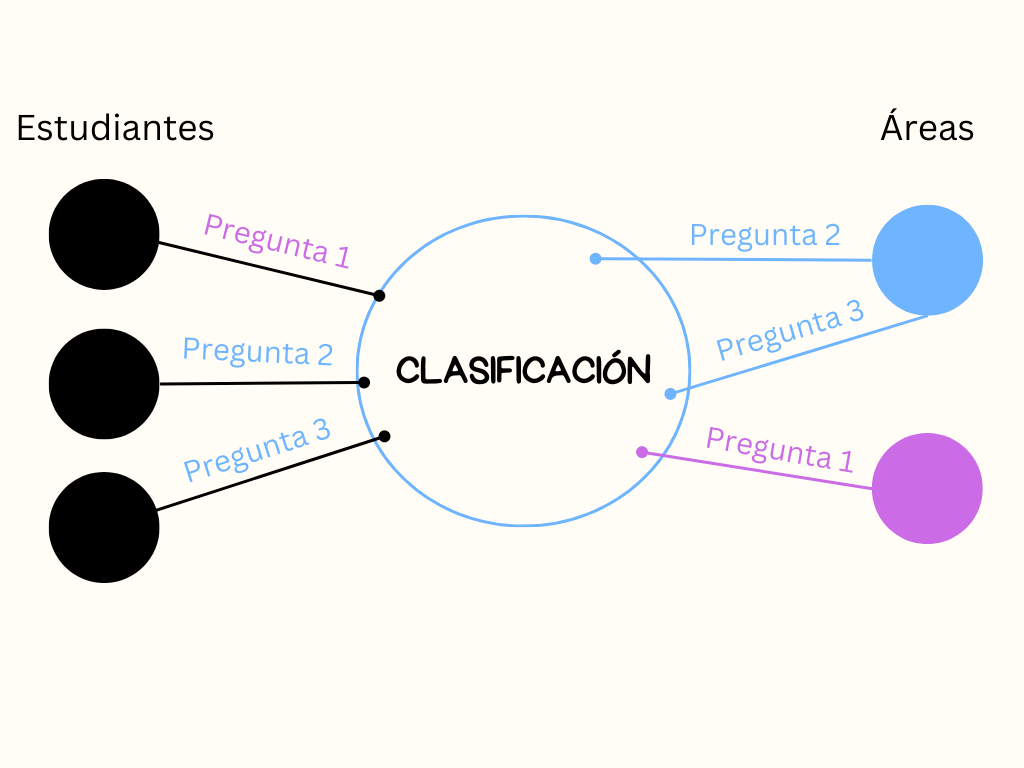
\includegraphics[width=15cm, height=11.25cm]{clasification.png}
	\caption{Mecanismo de clasificación}
	\label{fig:clasification}
\end{figure}

\begin{figure}[h]
	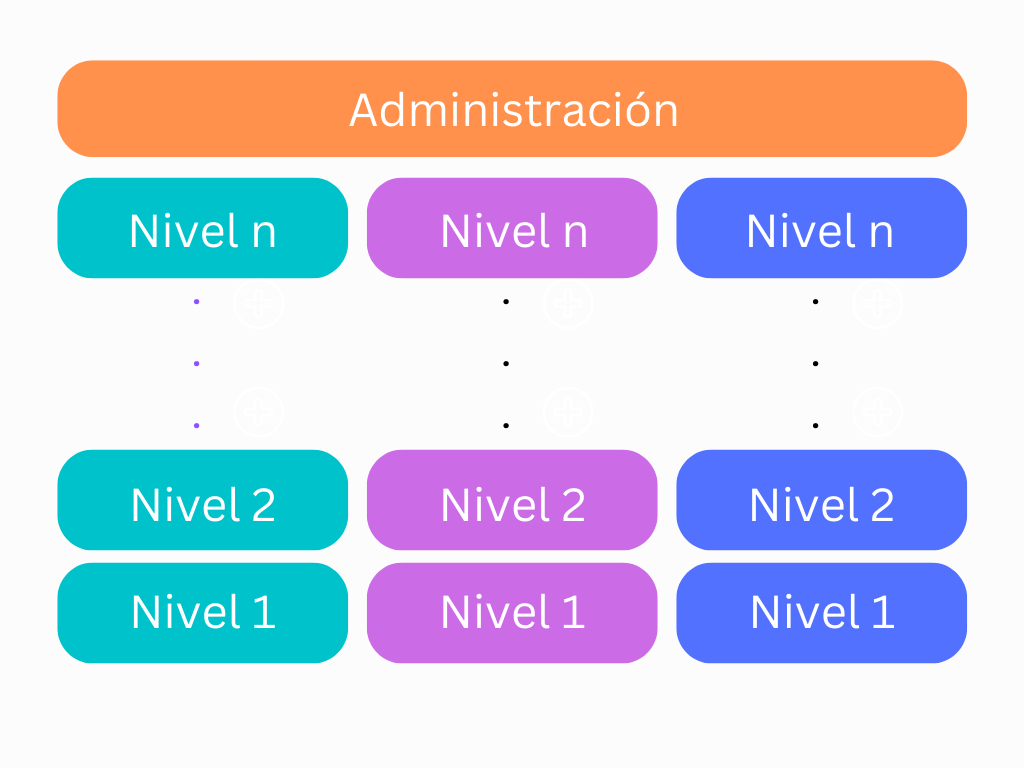
\includegraphics[width=15cm, height=11.25cm]{hierarchy.png}
	\caption{Jerarquía}
	\label{fig:hierarchy}
\end{figure}


\begin{figure}[h]
	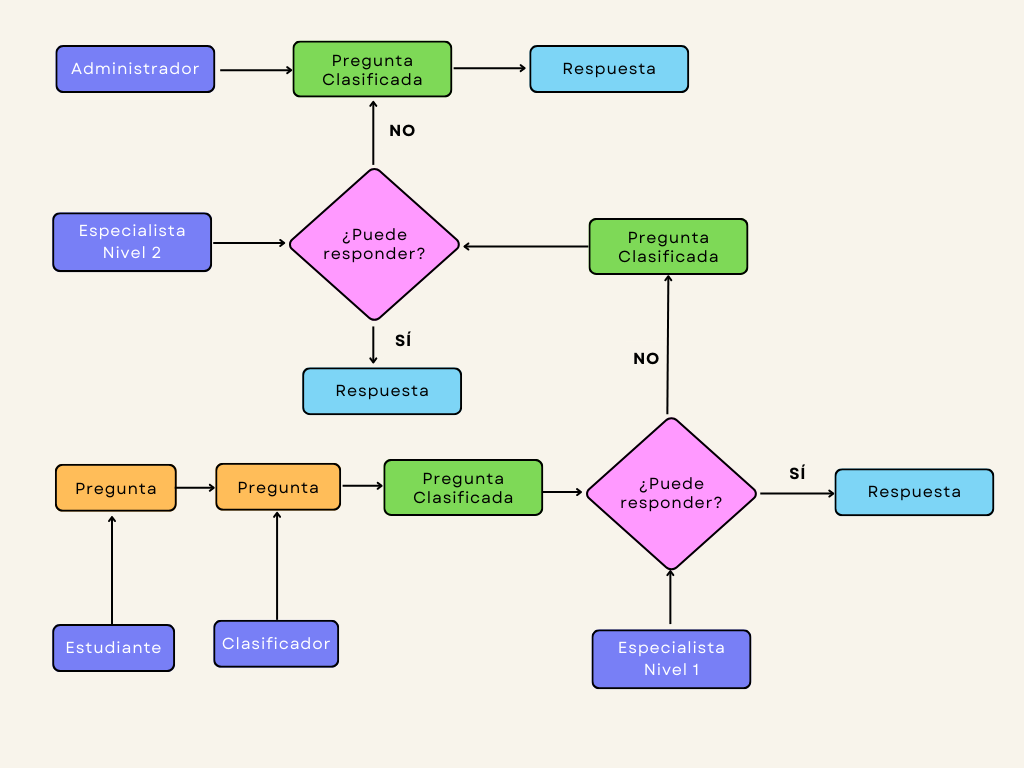
\includegraphics[width=15cm, height=11.25cm]{thesis_diagram.png}
	\caption{Propuesta del sistema}
	\label{fig:myprop}
\end{figure}



\chapter{Detalles de Implementación y Experimentos}\label{chapter:implementation}

El proyecto está compuesto por una REST API desarrollada en \href{https://gin-gonic.com/}{Gin} y un frontend desarrollado con \href{https://nuxtjs.org/}{Nuxt.js}.
\newline

Para el backend se usará una base de datos \href{https://www.postgresql.org/}{PostgreSQL} que será manejada a través del \textit{ORM} \href{https://gorm.io/}{Gorm}, se usará un sistema de \textit{JWT} para la autenticación, y los tokens de los usuarios se almacenarán en memoria usando una base de datos \href{https://redis.io/}{Redis}.
\newline

Para el frontend estaremos usando la \href{https://nuxtjs.org/}{Nuxt.js} en su versión 3.0, y nos apoyaremos de \href{https://tailwindcss.com/}{Tailwind CSS} para estilizar las vistas.

\section{Estructura de la Base de Datos}
\subsection{Tabla roles}

\begin{itemize}
	\item \textbf{id} (llave primaria, int)
	\item \textbf{name} (str)
\end{itemize}

\subsection{Tabla areas}

\begin{itemize}
	\item \textbf{id} (llave primaria, int)
	\item \textbf{name} (str)
\end{itemize}

\subsection{Tabla users}

\begin{itemize}
	\item \textbf{id} (llave primaria, int)
	\item \textbf{name} (str)
	\item \textbf{email} (str)
	\item \textbf{password} (str)
	\item \textbf{role\_id} (llave foránea (roles), int)
	\item \textbf{area\_id} (llave foránea (areas), int)
\end{itemize}

\subsection{Tabla statuses}

Las preguntas enviadas por los estudiantes pueden estar en un estado determinado:

\begin{itemize}
	\item \textbf{enviada:} el estudiante envió la pregunta y nadie ha interactuado con esta.
	
	\item \textbf{clasificada nivel 1:} un clasificador clasificó la pregunta en un área determinada.
	
	\item \textbf{clasificada nivel 2:} un especialista nivel 1 que se había hecho responsable la pregunta, no pudo responderla y la elevó al nivel 2.
	
	\item \textbf{clasificada admin:} un especialista de nivel 2, que se había hecho responsable de la pregunta que había sido previamente elevada al nivel 2, no pudo responderla y la elevó a la administración.
	
	\item \textbf{resuelta:} un especialista de nivel 1, de nivel 2, o un administrador respondió la pregunta.
	
\end{itemize}

Estos estados se encuentran almacenados en la tabla \textbf{statuses}, que tiene la siguiente estructura:

\begin{itemize}
	\item \textbf{id} (llave primaria, int)
	\item \textbf{description} (str)
\end{itemize}

\subsection{Tabla questions}

\begin{itemize}
	\item \textbf{id} (llave primaria, int)
	\item \textbf{text} (str)
	\item \textbf{response} (str)
	\item \textbf{status\_id} (llave foránea (statuses), int)
	\item \textbf{user\_author} (llave foránea (users), int)
    \item \textbf{user\_responsible} (llave foránea (users), int)
\end{itemize}

\subsection{Tabla message\_chats}

\begin{itemize}
	\item \textbf{id} (llave primaria, int)
	\item \textbf{text} (str)
	\item \textbf{readed} (boolean)
	\item \textbf{question\_id} (llave foránea (questions), int)
	\item \textbf{user\_id} (llave foránea (users), int)
\end{itemize}

\section{Backend}

\subsection{Estructura:}
El backend se estructura por capas:
\newline

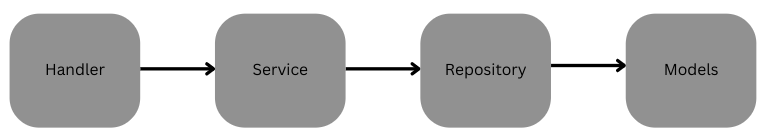
\includegraphics[width=13.8cm, height=2.5cm]{structure_backend.png}

La capa \textbf{Handler} es la encargada de interceptar los requests, interactuar con los permisos, detectar posibles errores dentro del request recibido, preparar las estructuras necesarias para finalmente ejecutar alguno(s) de los servicios de la capa \textbf{Service} para luego retornar el response adecuado para el request.
\newline

La capa \textbf{Service} consta de varios servicios tales como iniciar sesión, registrarse, etc, esta se encarga de ejecutar los pasos necesarios para la acción requerida, abstrayéndose de las validaciones del requests (porque ya fue hecho por la capa \textbf{Handler}), para obtener datos deberá pedírselos a la capa \textbf{Repository} y luego retornarlos a la capa \textbf{Handler}.
\newline

La capa \textbf{Repository} es la encargada de las operaciones con la base de datos, para ello recibe indicaciones de la capa \textbf{Serivice} y auxiliándose del \textit{ORM} \href{gorm.io}{Gorm} y inserta, modifica, lee, y/o elimina datos y le entrega una respuesta a la capa \textbf{Service}.
\newline

La capa \textbf{Models} tiene, con la sintaxis de estructuras de \href{go.dev}{Go}, se describen todas las entidades y las relaciones de la base de datos, para ello hace uso del \textit{ORM} \href{gorm.io}{Gorm}.


\backmatter

\begin{conclusions}
    De los principales softwares de reportes e incidencias existentes en el mercado, ninguno se adecuaba a los propósitos de la Universidad, por lo que se desarrolló desde cero una plataforma que puede ser editada en un futuro si se estima pertinente, se utilizaron algunas de las tecnologías punteras en la actualidad, es de fácil uso, tanto para el personal calificado como para los estudiantes. Al ser una solución web puede es accesible desde cualquier lugar con un dispositivo conectado a internet. Con ella se soluciona el problema de organización existente en los grupos de Telegram y Whatsapp, las dudas llegan a las personas capacitadas para darles respuesta y los especialistas más experimentados ahorran tiempo que pueden dedicar a las dudas más complicadas al no recibir incidencias comunes que pueden ser solucionadas por personal menos experimentado. 
\end{conclusions}

\begin{recomendations}
    El software desarrollado fue sometido a varias pruebas y pasó todas con éxito, aún así toda pieza de software está expuesta a posibles errores por lo que al lanzarse la plataforma se recomienda monitorear su funcionamiento ante posibles fallos que puedan ocurrir.
    \newline
    
    Es importante mantenerse informado en los avances que puedan existir en materia de desarrollo de software y de sistemas parecidos en el mundo, para poder adaptar la plataforma con las innovaciones que vayan saliendo a la luz y tener el mejor producto posible para los estudiantes de la universidad.
    \newline
    
    Acumular los datos para en un futuro tener material y poder entrenar modelos de inteligencia artificial para automatizar tareas como la clasificación de dudas y la respuestas a preguntas repetitivas. Es recomendable también mirar las tendencias de machine learning porque es un campo que está creciendo muy rápido y van a surgir tecnologías cada vez más potentes que pueden ser utilizadas apara mejorar el rendimiento del sistema.
\end{recomendations}

\printbibliography[heading=bibintoc]
\begin{thebibliography}{X}
	\bibitem{apirest} Documentación de Integración de Aplicaciones de Amazon
	
	
	\url{https://aws.amazon.com/es/what-is/api/#:~:text=API%20significa%20%E2%80%9Cinterfaz%20de%20programaci%C3%B3n,de%20servicio%20entre%20dos%20aplicaciones.}


	\bibitem{frontend_vs_backend} Qué es Frontend y Backend: diferencias y características - Platzi
	
	\url{https://platzi.com/blog/que-es-frontend-y-backend/}
	
	\bibitem{encuesta2022} Encuesta de StackOverflow 2022
	
	
	\url{https://survey.stackoverflow.co/2022/#most-popular-technologies-webframe}
	
\bibitem{vue} Documentación oficial de Vue

\url{https://vuejs.org/guide/introduction.html}

\bibitem{nuxt} Documentación oficial de Nuxt 3

\url{https://v3.nuxtjs.org/guide/concepts/auto-imports}

\bibitem{golang} Documentación oficial de Go

\url{https://go.dev/doc/}

\bibitem{gin} Documentación oficial de Gin

\url{https://gin-gonic.com/docs/}

\bibitem{postgres} Página oficial de PostgreSQL

\url{https://www.postgresql.org/}
	
\end{thebibliography}

\end{document}